% latexmk -pvc -pdf
\documentclass[a4paper, twocolumn]{article}
\usepackage[margin=0.65in]{geometry}
\usepackage{amsthm,amsfonts,amssymb}
\usepackage[english]{babel}
\usepackage{blindtext}
\usepackage{sidecap}
\usepackage{caption}
\usepackage{subfig}
\usepackage{graphicx}
\newenvironment{Figure}
    {\par\medskip\noindent\minipage{\linewidth}}
    {\endminipage\par\medskip}
\newenvironment{itemizeReduced}{
\begin{list}{\labelitemi}{\leftmargin=1em}
\setlength{\itemsep}{1pt}
\setlength{\parskip}{0pt}
\setlength{\parsep}{0pt}}{\end{list}
}

\title{
    
}
\author{Ana C. Fabela Hinojosa \\
\small{School of Physics and Astronomy, Monash University}}
\date{Last edit: \today}

\begin{document}
% \onecolumn
% \twocolumn
\maketitle

\begin{abstract}
This experiment aims to describe the observed spectra of photons emitted during the decay of a radioactive Cobalt source (\textsuperscript{57}Co),
by analysing the Mössbauer absorption spectrum of two distinct samples, I was able to determine the linewidth $\Gamma_v = 0.293\pm0.003$mm/s and isomer shift  $\textrm{IS}_{\rm KFCN} = (-0.1565\pm0.0013)$mm/s between a potassium ferrocyanide (KFCN) sample and a gamma particle source. In addition, I calculate the isomer shift for an alpha-Iron sample relative to the source ($\alpha$Fe): $\textrm{IS}_{\rm \alpha} = (-0.1253\pm0.0018)$mm/s by calibrating the velocity scale for the experiment. Using these results I obtained a relative isomer shift for both samples $\textrm{IS}_{rel} = -0.031\pm0.002$mm/s.
In this analysis I also deduce the nuclear angular momentum quantum number $I_e = 3/2$ and magnetic moment of the excited state of the KFCN sample $\mu_e = (-0.1537\pm0.0008)\mu_N$. Which corresponds to the $14.4$keV level of \textsuperscript{57}Fe.
\end{abstract}


\section{Introduction}
In 1961 Rudolf Mössbauer received the nobel prize for the discovery of a phenomenon presently known as the Mössbauer effect \cite{2}.
Mössbauer studied the resonance effects in the nuclei present in solid samples of Iridium. From his observations, he proposed that when atoms are bound in a solid, under certain circumstances a fraction of the nuclear events could occur without recoil. He attributed the observed resonance to the recoil free fraction $f$ of nuclear events\cite{0}.

% It is possible to observe very narrow linewidth nuclear transitions. Consequently this enables us  to see the hyperfine energy splittings of the nucleus caused by interactions with surrounding electrons\cite{0}. 

\section{Background Theory}
The decay process undergone by the radioactive \textsuperscript{57}Co source is primarily due to electron capture\cite{0}.
\begin{equation} Co^{57}_{27} + e^{0}_{-1} \rightarrow Fe^{57}_{26},
\end{equation}
where the resultant $Fe^{57}_{26}$ atom is in a excited state.
\subsection{Recoil energy}
After the electron capture event, the excited iron atom will emmit a $\gamma-$ray spontaneously. This $\gamma-$ray emission will classically result in recoil motion of the electron in opposite direction to the $\gamma-$ray emission, causing the atom to transition from an excited state to the ground state\cite{2}.
\begin{equation} E_R = \frac{E_{\gamma}^2}{2 m_R c^2}
\end{equation}
where $E_{\gamma}$ is the energy of the $\gamma-$ray, $m_R$ is the mass of the emitting nucleus and $c$ is the speed of light.

Equation (2) describes the physics that lead Mössbauer to make his outstanding contribution. In this equation we can see clearly that as the recoiling mass increases, the recoiling energy decreases. If instead of using a single atom of mass $m_R$, we use a crystal lattice of $n$ atoms we will approach the limit where we have zero recoil energy\cite{2}.

Electromagnetic theory tells us that the intensity of the transition $I(E)$, which is visible as an emission line follows the analytic form
\begin{equation} I(E) = \frac{(\Gamma / 2)^2}{(E - E_0)^2 + (\Gamma /2)^2}
\end{equation}
where $E_0$ is the centre and $\Gamma$ is the full width half maximum (FWHM) of the observed line.

In the introduction we mentioned the recoil free fraction of nuclear events $f$.
It is important to note that $f$ (ie. The fraction of recoil free nuclear events) is one of the most important parameters defining the usefulness of Mössbauer transitions\cite{8}.
Applying elementary theory to a Debye solid we find

\begin{equation} 
f = exp \left (\frac{-6 E_R}{k_B \Theta_D} \left (\frac{1}{4} + \left (\frac{T}{\Theta_D} \right)^2  \int_{0}^{\Theta_{D}/T} \frac{x}{e^x -1}dx \right )\right )
\end{equation}


where $\Theta_D$ is the Dabye temperature of the lattice (temperature at which the highest-frequency phonon mode is excited) \cite{13}, $T$ is the temperature at which the experiment is performed\cite{0} and $k_B$ is Boltzmann constant.

Equation (2) can be integrated numerically to produce a plot of $f$ as a function of $T$ for distinct values of $\Theta_D$\cite{8}.
In order to maximise $f$ : the ratio $\frac{E_R}{\Theta_D}$ should be minimised\cite{8}. 
This means that the optimal conditions for Mössbauer spectroscopy occur when 
\begin{itemizeReduced}
    \item The emitted photon energy $E_{\gamma} < 100$ keV. This condition is equivalent to $E_R$ being small,
    \item At room temperature: The Dabye temperature $\Theta_D$ should be large, ie. $~\Theta_D > 100$ K\cite{13},
    \item Absorbing nuclei must be in the ground state in order to achieve a transition\cite{10}\cite{13}.
\end{itemizeReduced}

\subsection{Obtaining a Mössbauer spectrum}
As the first item in the list above explains, the ideal experimental configuration to observe the Mössbauer effect requires $\gamma-$rays with energies that cover a specific energy range ($E_{\gamma} < 100$ keV). To satisy this condition experiments use mechanisms that physically move the source of $\gamma-$rays in order to Doppler shift the emitted photons\cite{10}. The energy shift of the $\gamma-$rays due to the Doppler effect is
\begin{equation} \Delta E = E_{\gamma} \frac{v}{c}
\end{equation}
where $E_{\gamma}$ is the $\gamma-$ray rest frame energy, $v$ is the velocity of the $\gamma-$ray source and $c$ is the speed of light.

The natural linewidth of the $14.4$keV transition is only $4.67 \times 10^{-9}$ eV\cite{0}. A doppler shift of $1\times10^{-4}$m/s corresponds to this energy\cite{0}.


%PAGE 4?

\section{Method}
\subsection{The Mössbauer Drive system}
The experimental set-up allows the user to obtain a range of $\gamma-$ray energies. A transducer containing a driving coil and a pick up coil is used to move the source back and forward to achive the Doppler shift in $\gamma-$ray energies. The pick-up coil produces a signal that is proportional to the actual velocity and hence used as a reference signal\cite{0}.
The velocity of the sample changes linearly driven by the transducer, this motion requires constant acceleration $a$ for the first half of the cycle, and a constant acceleration of equal magnitude to $a$ but in opposite direction during the second half of the cycle\cite{0}.
Under these conditions, the multichannel analyser (MCA) used to observe the driving signal of the transducer displays a triangular signal for the velocity. 
This triangular signal and the reference signal from the pick-up coil may differ by an error signal, which is amplified, inverted and fed back in as part of the drive signal. The error signal is then monitored on the digital storage oscilloscope (DSO) as well as on the bar graph display on the MR-260 drive unit used to control the motion of the transducer\cite{0}.

Each channel corresponds to equal velocity increments\cite{0}. After the counting of emmited rays is finished and once the spectrum is obtained, one must use the software provided to fold the resultant spectrum, since the image obtained is a mirror image of the actual measured spectrum of energies\cite{0}.

\subsection{Data Aquisition}
Since I did not do the experiment I will simply give a description of the process for the reader.
Caution must be taken since the source is quite strong (1-2 mCi) The experimenter will need a radiation dosimeter and the key to the source box (obtained from the laboratory preparation room) before starting the experiment\cite{0}.
In order to minimise risk of exposure, the experimenter must leave the lead cover on the source at all times except when strictly necessary.
The experimenter must not touch the source.

First, the experimenter should turn on all the equipment. The box that houses the source must be unlocked and the side catches must be released. After opening the front one must verify that the radioactive source is mounted in the transducer. If this is not the case a demonstrator will help the experimenter fix this. Two absorber samples are mounted on persplex slides. If one of the absorber samples is in front of the source, remove the absorber sample and place it in the holder on the left handside of the box.

\subsection{Observing the pulse height of the $\gamma-$spectrum}
The experimenter must plug the output of the amplifier into CH1 of the DSO, and examine the pulses which should be unipolar with a maximum height of ~6-8 V\cite{0}. If these conditions are not satisfied, the experimenter should adjust the amplifier gain, since the pulse height behaves linearly with respect to the energy of the photons detected\cite{0}. 

The experimenter should familiarise themself with the decay scheme of \textsuperscript{57}Co in order to identify the features visible in the spectrum. The top bright band in the spectrum corresponds to $122$keV and $137$keV $\gamma-$rays\cite{0}. These rays have poor resolution by the scintillation detector on their compton and scape peaks. The second bright band visible corresponds to the desired transition of $14.4$keV $\gamma-$rays. Lastly the $6.3$keV iron K x-rays are nearly entirely absorbed by the Be window of the detector and hence lost in the noise\cite{0}. The data acquisition hardware is set to MCA mode.

To observe the pulse-height spectrum of the signal the experimenter must click on the Windows “Start” menu and select “Computer” then "OS Disk C", and finally click on Program Files (X86), Wissel, Wissoft 2010, to execute "Wissoft.exe". This will open a new window of the software.
Clicking on the central icon (USB Q-74-0615) will make another window appear showing the last captured spectrum\cite{0}. 

The experimenter must click on the “Settings” in the “Device” menu (lower “Settings”)and set the options to configuration displayed in Figure 1. below

\begin{figure}[h]
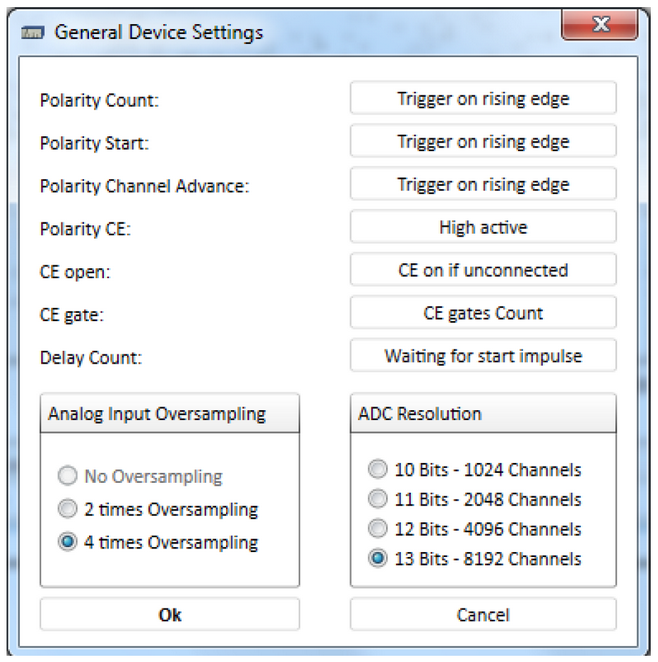
\includegraphics[width=0.5\textwidth]{general_device_settings.png}    
\caption{Specified general settings for the CMCA-550 data acquisition device\cite{0}.
}
\end{figure}

In the “Data Acquisition” menu, the experimenter must click “PHA” in the mode grouping, “Single” in the windows gouping and set the “Hysteresis” to 25mV\cite{0}. 
In the “Window 1” menu, the range should be set from 50mV to 9990mV. These settings  will allow the scale of the window to display the full pulse size\cite{0} and they will become active after the experimenter clicks "OK".  Before begining the acquisition, the experimenter must click “Clear Memory”, then click  “Start” to begin a new acquisition process.

A large signal for low channels will be visible in the spectrum (often visible in channels corresponding to less than 200mV). This effect is due to electrical noise and can be eliminated by increasing the low level range from 50mV to an appropriate level\cite{0}.
To correct the spectrum for the noise, the experimenter should click in the "Tools" menu, and then click “Set”. 
After this, they must click in the main display window at the upper edge of the region they wish to exclude (often greater than 200mV). These new settings are preserved by clicking “Save”\cite{0}.
To stop the acquisition the experimenter must click “Stop” and then “Clear Memory” and “Start” again with the adjusted region\cite{0}.

In the observed spectrum two consecutive peaks will be visible. As explained before, it is only the lower energy peak which corresponds to the desired observable transition of $14.4$keV gammas. Therefore, in order to focus the spectrum, the experimenter must repeat the previous steps to define an adequate upper bound for the visible spectrum. Note that the width of the peak observed in the energy spectrum is due to measurement effects in the detector ($>10$keV) and it is much wider than the energy spread that actually occurs in the transition\cite{0}.

\subsection{Mössbauer spectrum of potassium ferrocyanide}
\subsubsection{Activating the MCS mode}
Acquiring the Mössbauer spectrum, requires that that the experimenter observes the absorption of $14.4$keV gamma photons as they are Doppler shifted in energy, scanning over the absorption peak(s) in the sample\cite{0}.
In this experiment only the $14.4$keV gammas are counted; this count is plotted as a function of energy shift. To do this the experimenter must activate the Multi-Channel Scaler (MCS) acquisition mode\cite{0}.

\subsection{Data acquisition}
\subsubsection{Mössbauer spectrum of potassium ferrocyanide (KFCN)}
To observe the Mössbauer spectrum of KFCN, the experimenter must click on the top “Settings” menu followed by the “MCS [Window]” option.
From the top “Windows” menu, the experimenter must click on the “Single” option. The MCS acquisition is configured to use the values for the window from the previous PHA settings\cite{0}. The experimenter must verify that this is the case and proceed to click "OK".

The KFCN absorber is prepared using iron in which the \textsuperscript{57}Fe isotopic abundance has been increased from the natural $2.2\%$ to $70\%$\cite{0}. 
The experimenter must now open the source box and place the absorber in the holder that is in front of the source\cite{0}. The velocity range helipot on the front of the Mössbauer drive unit must be adjusted to 0.4 and the velocity switch below to “x0.1”\cite{0}. 

The magnitude of the velocity drive to the transducer is measured by connecting the DSO (CH1) to the “monitor” output of the MR-260A drive unit\cite{0}. The experimenter must determine the calibration factor for the measured velocities. This can be done quite accurately from measurements on the Mössbauer spectra\cite{0}The experimenter must record the the frequency and the peak-to-peak voltage (VPP), for this sample the $\textrm{VPP} \approx 160$mV. To get a sensible average the signal should be displayed for at least 10 periods, since the total signal is modified by the error signal continuously at the acceleration change points\cite{0}.

After clicking “Clear Memory”, and then “Start” the experimenter is free to begin with the data acquisition. 
For visualisation purposes, the experimenter should right click in the main display window and and select the “Full Range” option. This makes the MCS spectrum fill the display window. By clicking on the “Channels” button at the bottom of the window to display the spectrum in terms of MCS channels\cite{0}. 

The experimenter must check the error signal. This can be done by connecting the error output of the MR-260A drive unit to the DSO. The amplitude of the signal should be no more than a few tens of mV\cite{0}. The mean error value of the signal is displayed on the logarithmic bar-graph display. There are two sources of the error signal - the constant spikes where the acceleration changes sign and a non-phase-locked signal which is due to 50 Hz and is visible on the velocity signal\cite{0}. If the error signal should become very large this means that the drive has gone into oscillation, this issue can be resolved by tuning the feedback loop with the help of a demonstrator.

Since this is a nuclear counting experiment it is important to maximise the signal to noise ratio, therefore best results are obtained when the experiment is run for at least 3 hours. After a clear spectrum is obtained, saving the spectrum requires that the experimenter clicks the “Stop” button (this terminates the data acquisition). To save the raw spectrum, the experimenter must click "Save as" This saves the file as "specified-filename-here.unf" format.
The experimenter will observe that the raw spectrum is mirrored around one of the maximum velocity points (channel 512)\cite{0}. In order to improve the signal to noise ratio, the spectrum must be “folded”. This process removes geometrical distortion due to the changing solid angle subtended at the source by the detector. The experimenter should click on the “Folding” button on the “Mössbauer Velocity Calibrator Tools” menu and save the resulting spectrum (as .fld) for subsequent fitting to determine the various parameters of the data\cite{0}.

\subsubsection{Mössbauer spectrum of $\alpha-$Iron}

For this part, the experimenter must replace the KFCN absorber with the metallic iron absorber and only change the velocity control helipot to 1.80 (keeping the velocity range switch on “x0.1”). After these steps, the experimenter must record the actual amplitude of the scan voltage (VPP) by measuring the p-p voltage on the “monitor” output of the drive unit. The VPP value should be approximately $720$mV\cite{0}.

Note that the iron is below its Curie temperature and hence has an internal magnetization which is proportional to the time average value of Jz (for the electrons). The nucleus interacts with the electron cloud in this configuration as an effective magnetic field at room temperature of of value $33.04$T, this is known as magnetic hyperfine field. Under this conditions the atomic level splitting is described by the Zeeman effect. Under these conditions the experimenter will observe a 6 line spectrum\cite{0}\cite{8}.
To maximise the signal to noise ratio, this part of the experiment should run at least overnight. The experimenter must record the velocity range using the DSO and verify that the error signal is well below $1\%$\cite{0}.

When the data acquisition is finalised, the experimenter must repeat the steps followed in the Mössbauer spectrum of KFCN to save both the raw spectrum and the folded version as different files for later analysis\cite{0}.

\subsection{Spectrum fitting}
The analytical lineshape for a decaying quantum system is a Lorentzian\cite{0}
In the case of the KFCN spectrum I use the following equation as the model
\begin{equation} I(E) = B - \frac{A(\frac{\Gamma}{2})^2}{(E - E_0)^2 + \frac{\Gamma^2}{4}},
\end{equation}
where $E$ is the corresponding MCA channel number, $B$ is the background count (baseline), $E_0$ is the channel number corresponding to the centre of the visible dip, $A$ is the depth of the dip in counts, from the baseline and $\Gamma$ is the linewidth (FWHM) in channels\cite{0}.
This model has 4 paramaters to minimise.

To fit the Mössbauer spectrum of $\alpha$Fe, 6 absorption lines are required, so the model becomes
\begin{equation} I(E) = B - \sum_{i=1}^{6}\frac{A_i(\frac{\Gamma_i}{2})^2}{(E - E_{0,i})^2 + \frac{\Gamma_{i}^2}{4}},
\end{equation}
This model is similar to the KFCN model, with the exception that we have now 6 dips, each dip in the spectrum has 3 intrinsic parameters to minimise. Since we are including the baseline $B$ as a parameter of our model, the number of parameters to minimise in this model is 19.

\clearpage
% \twocolumn
\onecolumn
\section{Results}
\subsection{Data acquisition parameters}
As provided by the experimenter.
\begin{itemizeReduced}
    \item KFCN VPP$=160\pm1$mV
    \item $\alpha$-Fe VPP$=711\pm2$mV
\end{itemizeReduced}

%-----------Q6
Using equation (2) I found the recoil energy of a free iron nucleus after emitting a $14.4$keV photon$ E_R = 1.99$meV. 
This value is much smaller than the known chemical binding energy of the atom in the solid $BE = 7.024$eV\cite{11}

To compare $E_R$ to phonon energies, I estimated the longest wavelength phonon that can exist parallel to the gamma direction in the 6 \textrm{$\mu$}m thick source foil. By assuming the velocity of sound in metals as $\approx 1\times104$m/s\cite{0}. I estimated the resultant phonon energy to be $E_p = 3\times10^3$meV. Then, the phonon energy is much smaller than the recoil energy.

From these comparisons I concluded that the recoil energy produced by the gamma emmision will not remove an iron atom from an iron crystal, and consequently  a large fraction of the recoil energy will be lost to the crystal environment.
% -----------Q7
The ground state and the $14.4$keV excited level are respectively split into sublevels defined as the Zeeman effect describes. From the quantum mechanical selection rules for allowed dipole transitions ie. $\Delta$m$=0$ or $\Delta$m$=\pm1$. I deduced that the angular momentum of the excited state $I_e = \frac{3}{2}$. 

% -----------Q8
\begin{figure}[!htbp]
\subfloat[]{\scalebox{0.2}{
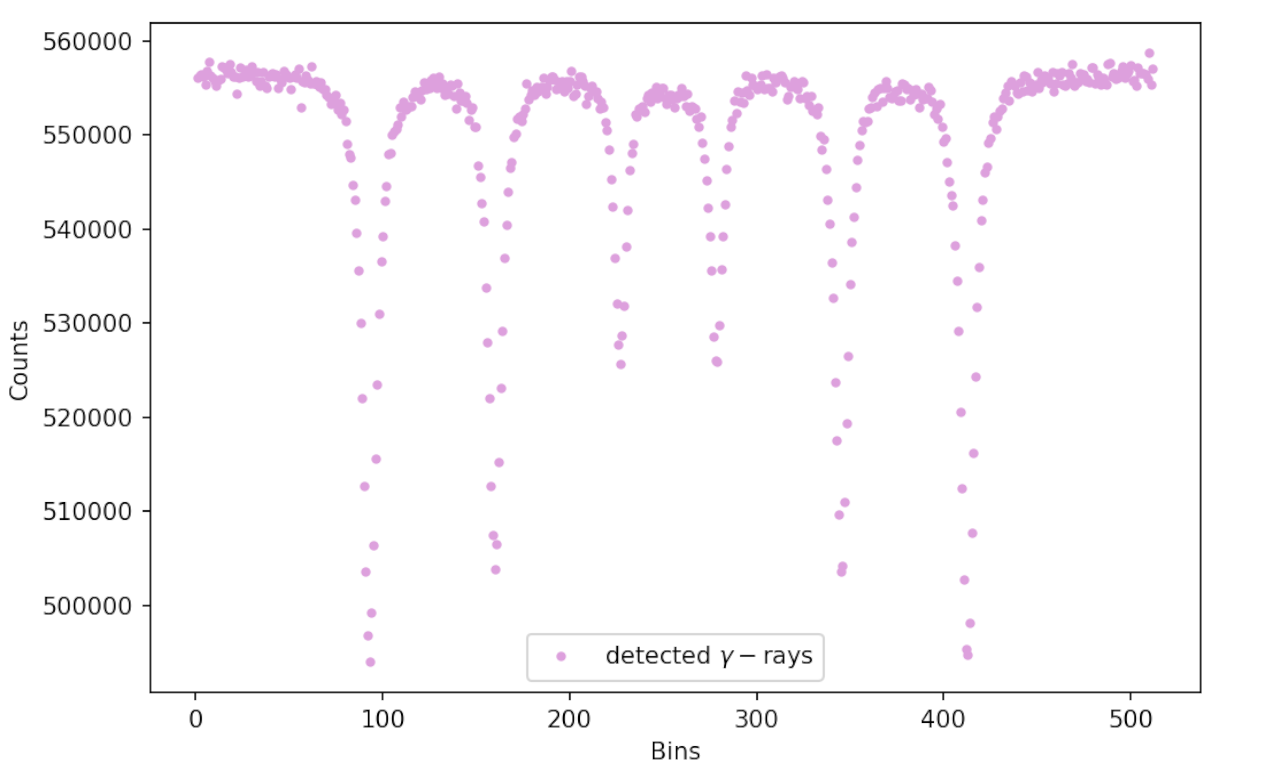
\includegraphics{alpha_folded.png}    
}}
\subfloat[]{\scalebox{0.2}{
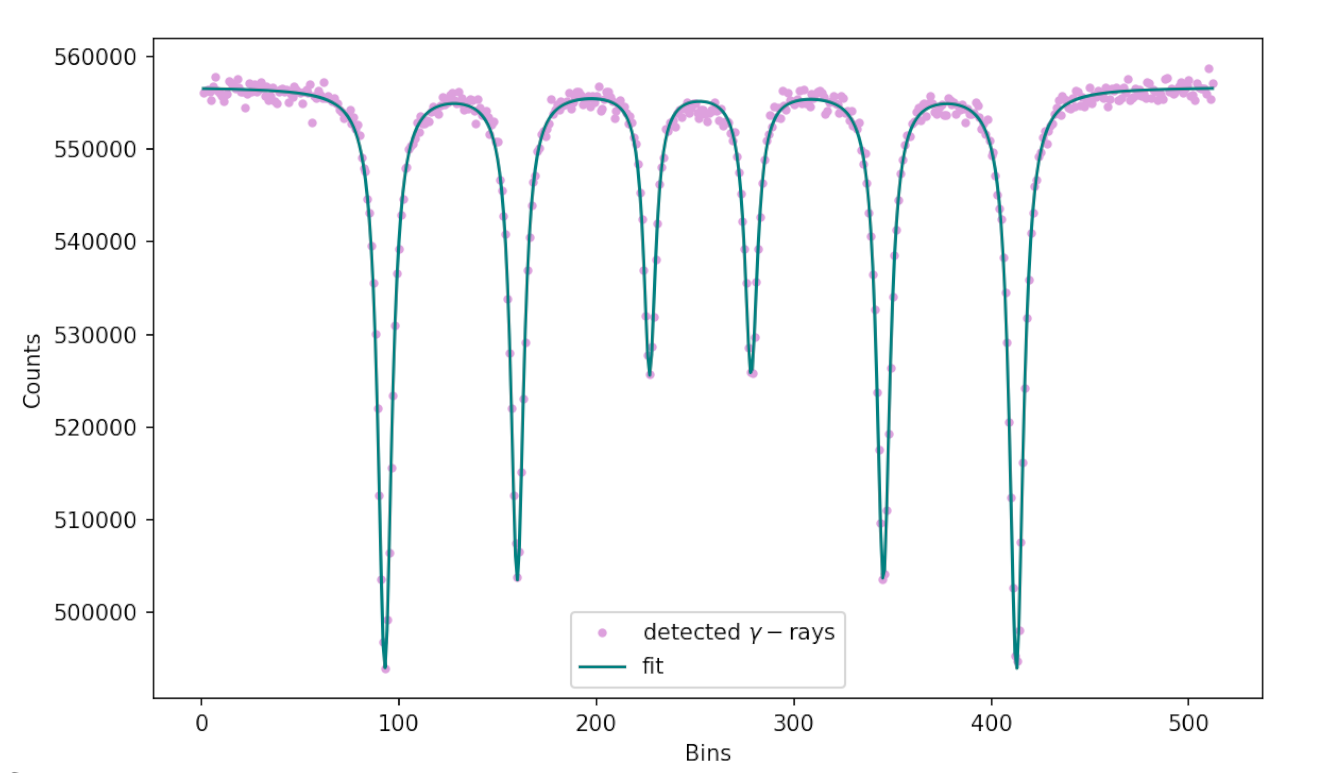
\includegraphics{alpha_fitted.png}   
}}
\caption{(a)Raw absorption spectrum of $\alpha$-Iron\\ 
(b) Fitted spectrum of $\alpha$-Iron using a 6 lorentzian sum model (the fit is done using 19 parameters).
}
\end{figure}

I calculated the energy of the ground state splittings to be $E_{g,1} = -1.51\times10^{-26}$J and $E_{g,2} = 1.51\times10^{-26}$J both values have an uncertainty of $8\times10^{-36}$. These values show that the ground state magnetic moment is positive.

I identified two pairs of possible transitions (ie. absorption lines) separated by two independent values for the distance between the ground state splittings. to find these, I verified the symmetry of the $\alpha$Fe spectrum using the fit results for the dip centres and the energy difference (channel units) between adjacent absorption dips. From this analysis I deduced that the distances between the ground state splittings are $\Lambda_{g,1} = 118.39\pm 0.06$ channels and $\Lambda_{g,2} = 118.48\pm 0.06$ channels. After some visual analysis I was able to determine that the magnetic moments of the ground state and the excited state have different signs.

The calculation for the magnetic moment of the ground state yielded $\mu_g = 4.5\times10^{-28}$J/T with an uncertainty of $1.4\times10^{-37}$J/T. Consequently, the ratio $g_g = \frac{\mu_g}{\mu_N I_g} = 0.18080000000\pm 0.00000000008$. Using these results I found that the total distance between ground state energy splittings is $\Lambda_g = 1.88316\pm 0.00003\times10^{-7}$eV.

By using $\Lambda_g$ in place of $\Delta E$ in the Doppler shift formula, I was able to calculate the velocity $v = 3.92\pm0.01$mm/s which will be used in the calibration constant for the spectrum. This calibration allows us to find the natural linewidth of a transition. The calibration constant found is $K_{1.8} = 0.0331\pm0.0001$mm/s/channels.




The spectrum of $\alpha$Fe has 4 independent measures for the excited state energy splitting separations ($\lambda_i$). I calculated a mean value for $\lambda$ using the parameters from my fit to the spectrum. The resultant mean separation is $\mu_{\lambda} = 67.12\pm0.03$ channels.

From my fit I obtained the energy of the excited state splittings (in channel units). Using $\mu_{\lambda}$ and $K_{1.8}$ I calculated the mean velocity $v_{\mu} = 2.222\pm0.008$mm/s, and once again, by using the doppler shift formula I calculated the energy separation between the splittings of the excited state in energy units: $\Delta E = (1.710\pm0.008)\times10^{-26}$J. I used this result to find the excited state g-factor $g_e = -0.1025\pm0.0005$. I declared this result to be negative since the exited state moment is negative.




The magnetic moment of the excited state was found to be $\mu_e = (-0.1537\pm0.0008)\mu_N$.
% -----------Q9
\begin{figure}[!htbp]
\centering
\subfloat[]{\scalebox{0.205}{
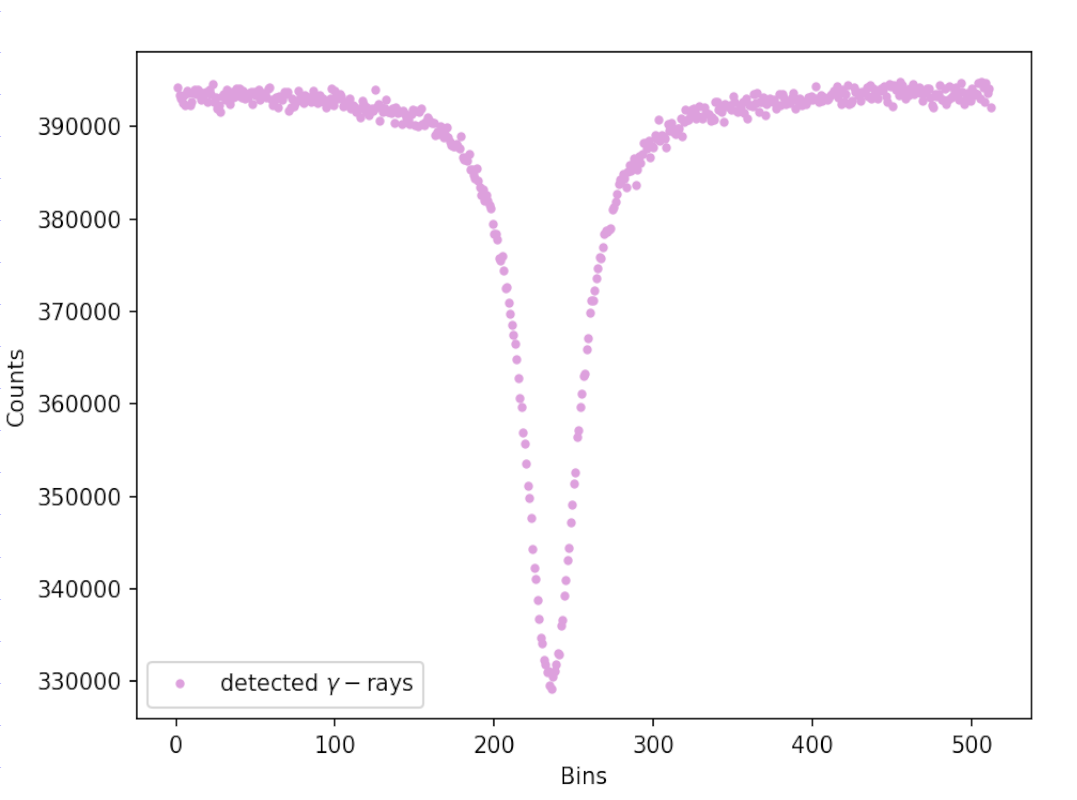
\includegraphics{KFCN_folded.png}    
}}
\subfloat[]{\scalebox{0.21}{
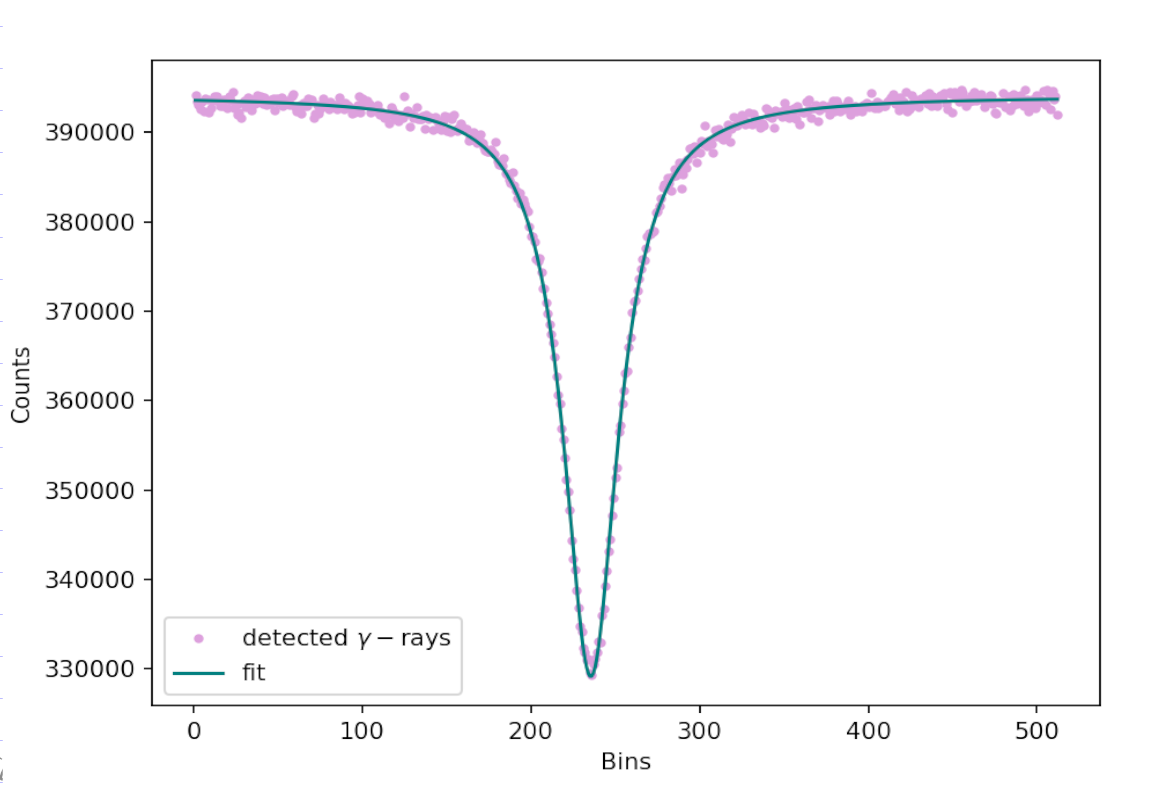
\includegraphics{KFCN_fitted.png}   
}}
\caption{(a)Raw absorption spectrum of Potassium ferrocyanide\\ 
(b) Fitted spectrum of Potassium ferrocyanide.
}
\end{figure}
From my previous results for $K_{1.8}$ and the ratio of the VPPs for both absorbers, the calibration constant for the KFCN spectrum was calculated to be $K_{0.4} = 0.00745\pm0.00006$mm/s/channel.
From this calibration, I calculated the converted linewidth $\Gamma_v = 0.293\pm0.003$mm/s for the KFCN spectrum.

 % -----------Q10
To determine the isomer shift of KFCN with respect to $\alpha$Fe, I defined the channel at the center of both spectra as $C_0$. Given the channel range I used [1-512], I determined that $C_0 = 256.5\pm0.05$

To continue with the isomer shift calculation, I split the process into two steps.
First step: I found the isomer shift of KFCN with respect to the source.
To do this I determined the centre of the absorption line from my fit to the spectrum: $C_{\rm KFCN} = 235.49\pm0.07$ channels.
The result for this isomer shift is $\textrm{IS}_{\rm KFCN} = -0.1565\pm0.0013$mm/s.

Second step: I determined the isomer shift of $\alpha$Fe with respect to the source in a similar way to the KFCN spectrum. 
The centre of the spectrum dips was found by taking an average of every energy transition in the spectrum \\$C_{\rm \alpha} = 252.713\pm0.016$ channels which lead me to find the isomer shift for $\alpha$Fe: $\textrm{IS}_{\rm \alpha} = -0.1253\pm0.0018$mm/s.




In order to find the isomer shift of KFCN with respect to $\alpha$Fe I subtracted their respective isomer shifts:
$\textrm{IS}_{rel} = -0.031\pm0.002$mm/s. I compare this result to the reported result in E Murad, J Cashion(2004) $\textrm{IS}_{\rm MC} = -0.035\pm0.007$mm/s. By taking the difference between my result and their reported relative isomer shift, and progating the uncertainty in this difference. 
The number of sigma between my result and Murad and Cashion is found by dividing the difference by the propagated uncertainty.
From this process I was able to determine that my result is $0.5\sigma$ away from their reported result.

\begin{figure}[!htbp]
\centering
\subfloat[]{\scalebox{0.25}{
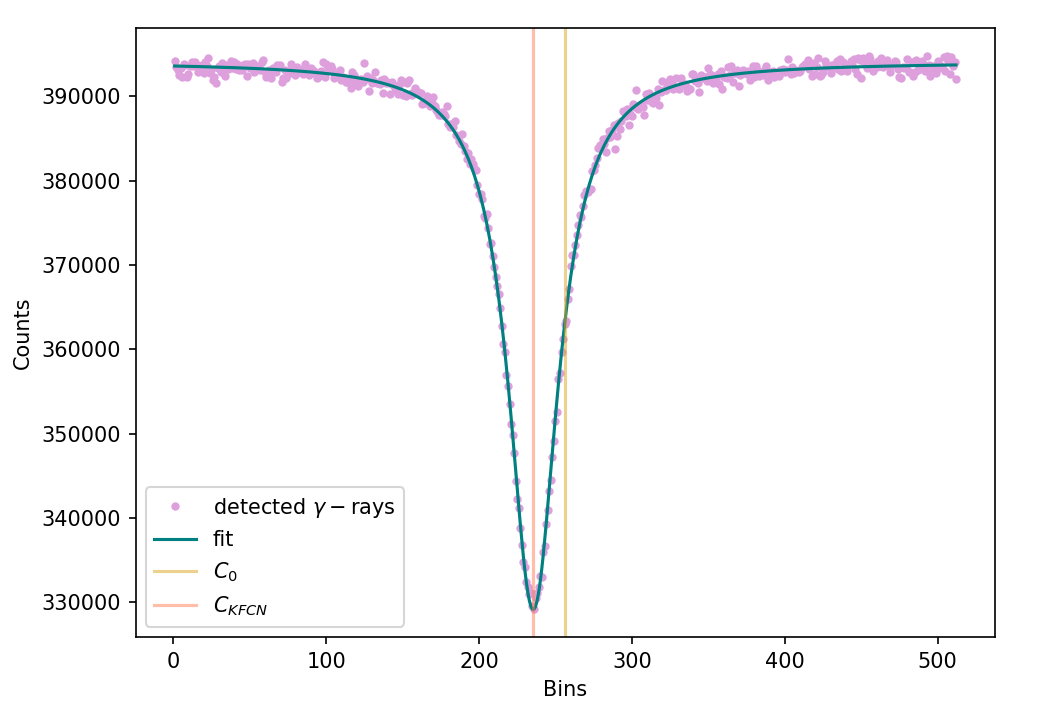
\includegraphics{centers_KFCN.png}    
}}
\subfloat[]{\scalebox{0.25}{
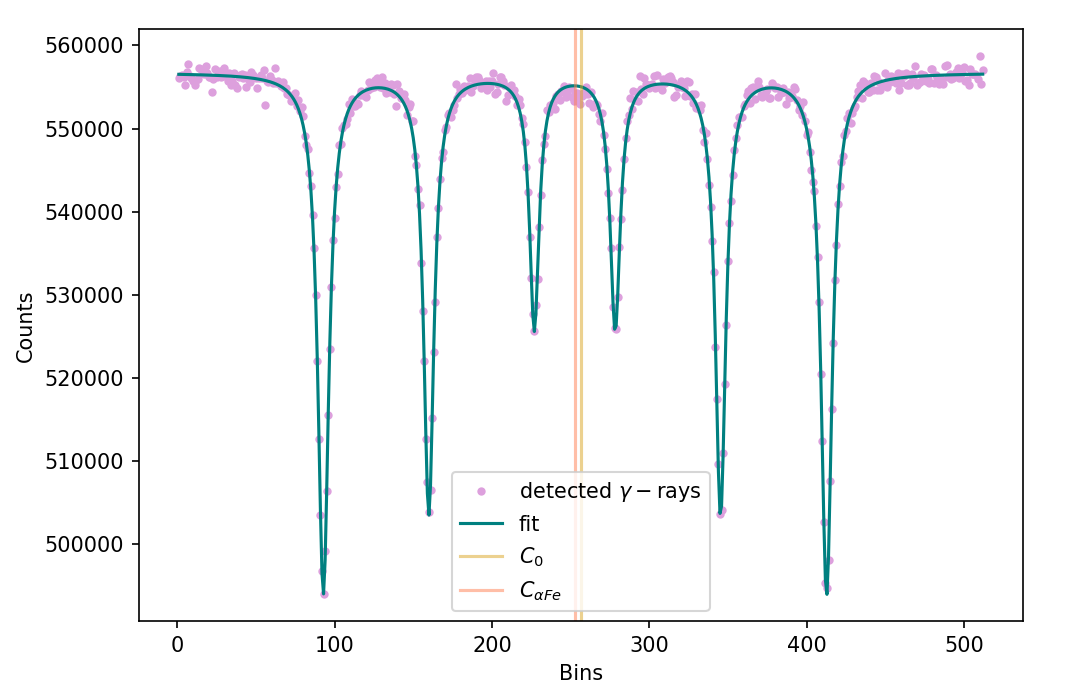
\includegraphics{centers_alpha.png}   
}}
\caption{(a) Fitted spectrum of Potassium ferrocyanide\\ 
(b)Fitted spectrum of alpha-Iron. Both plots include lines that mark the centres of the data in each spectrum ($C_{\rm KFCN}$ and $C_{\rm \alpha}$ respectively) in addition to a line that marks the absolute centre of the channel range used to plot the spectra ($C_0$).
}
\end{figure}

\begin{equation} 
\end{equation}

\clearpage
\twocolumn

\section{Discussion}

To fit both spectra I used the function optimize.curve\_fit from the SciPy library in Python.
This function is ideal for this type of analysis since it returns an array of optimal values for the parameters in the fit so that the sum of the squared residuals of the fit and the data is minimised\cite{15}. In addition, the function returns an estimated covariance matrix.

The optimize.curve\_fit function requires the specification of a boolean parameter (absolute\_sigma). If absolute\_sigma is set as False the affect on the returned covariance matrix is based on scaling standard deviations of errors in the data by a constant factor (sigma). This means that the constant sigma is set by demanding that the reduced $\chi^2$ for the optimal parameters of the fit is unity\cite{15}. Hence yielding a very adequate fit in most cases.

\section{Conclusion}
In this experiment I determine the linewidth $\Gamma_v = 0.293\pm0.003$mm/s and isomer shift $\textrm{IS}_{\rm KFCN} = -0.1565\pm0.0013$mm/s of the a potassium ferrocyanide sample and the isomer shift $\alpha$Fe: $\textrm{IS}_{\rm \alpha} = -0.1253\pm0.0018$mm/s of an alpha Iron sample by calibrating the velocity scale for the experiment. By using these results I obtain a relative isomer shift for both samples $\textrm{IS}_{rel} = -0.031\pm0.002$mm/s.
In addition, I deduce the nuclear angular momentum quantum number $I_e = 3/2$ and the magnetic moment $\mu_e = -0.1537\pm0.0008\mu_N$ for the excited state of a potassium ferrocyanide sample.

\bibliography{mybib}
\bibliographystyle{unsrt}
\end{document}